\documentclass[tikz,border=8pt]{standalone}
% Shared look for every TikZ diagram. Load with % Shared look for every TikZ diagram. Load with % Shared look for every TikZ diagram. Load with \input{../../tools/tikz-style.tex}
\usepackage[T1]{fontenc}
\usepackage{lmodern}
\renewcommand{\sfdefault}{lmr}  % diagrams use the same serif as the text
\usetikzlibrary{arrows.meta, positioning, shapes.geometric, calc, fit, backgrounds}
\definecolor{cblue}{HTML}{4C78A8}
\definecolor{corange}{HTML}{F58518}
\definecolor{cgreen}{HTML}{54A24B}
\definecolor{cred}{HTML}{E45756}
\definecolor{cpurple}{HTML}{B279A2}
\definecolor{cgrey}{HTML}{6B6B6B}
\tikzset{
  every picture/.style={font=\sffamily, line width=1.2pt},
  box/.style={draw=#1, fill=#1!12, rounded corners=4pt, align=center, inner sep=7pt, minimum height=1.1cm},
  box/.default=cgrey,
  arrow/.style={-{Stealth[length=3mm]}, draw=cgrey, line width=1.4pt},
  title/.style={font=\sffamily\bfseries\Large},
  note/.style={font=\sffamily\small, text=cgrey, align=center},
}
\AtBeginDocument{\hyphenpenalty=10000 \exhyphenpenalty=10000}

\usepackage[T1]{fontenc}
\usepackage{lmodern}
\renewcommand{\sfdefault}{lmr}  % diagrams use the same serif as the text
\usetikzlibrary{arrows.meta, positioning, shapes.geometric, calc, fit, backgrounds}
\definecolor{cblue}{HTML}{4C78A8}
\definecolor{corange}{HTML}{F58518}
\definecolor{cgreen}{HTML}{54A24B}
\definecolor{cred}{HTML}{E45756}
\definecolor{cpurple}{HTML}{B279A2}
\definecolor{cgrey}{HTML}{6B6B6B}
\tikzset{
  every picture/.style={font=\sffamily, line width=1.2pt},
  box/.style={draw=#1, fill=#1!12, rounded corners=4pt, align=center, inner sep=7pt, minimum height=1.1cm},
  box/.default=cgrey,
  arrow/.style={-{Stealth[length=3mm]}, draw=cgrey, line width=1.4pt},
  title/.style={font=\sffamily\bfseries\Large},
  note/.style={font=\sffamily\small, text=cgrey, align=center},
}
\AtBeginDocument{\hyphenpenalty=10000 \exhyphenpenalty=10000}

\usepackage[T1]{fontenc}
\usepackage{lmodern}
\renewcommand{\sfdefault}{lmr}  % diagrams use the same serif as the text
\usetikzlibrary{arrows.meta, positioning, shapes.geometric, calc, fit, backgrounds}
\definecolor{cblue}{HTML}{4C78A8}
\definecolor{corange}{HTML}{F58518}
\definecolor{cgreen}{HTML}{54A24B}
\definecolor{cred}{HTML}{E45756}
\definecolor{cpurple}{HTML}{B279A2}
\definecolor{cgrey}{HTML}{6B6B6B}
\tikzset{
  every picture/.style={font=\sffamily, line width=1.2pt},
  box/.style={draw=#1, fill=#1!12, rounded corners=4pt, align=center, inner sep=7pt, minimum height=1.1cm},
  box/.default=cgrey,
  arrow/.style={-{Stealth[length=3mm]}, draw=cgrey, line width=1.4pt},
  title/.style={font=\sffamily\bfseries\Large},
  note/.style={font=\sffamily\small, text=cgrey, align=center},
}
\AtBeginDocument{\hyphenpenalty=10000 \exhyphenpenalty=10000}

\begin{document}
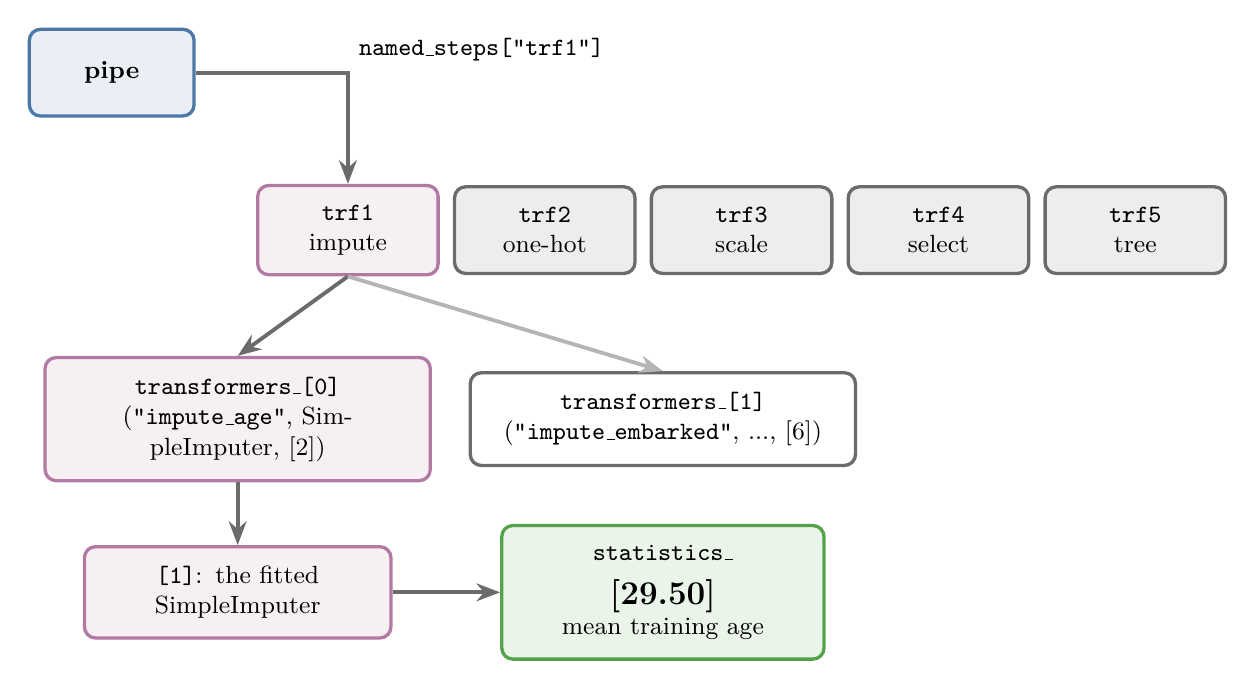
\begin{tikzpicture}[st/.style={box=#1, text width=3.0cm, font=\sffamily\small}]
  \node[st=cblue, text width=1.6cm] (p) at (0,0) {\textbf{pipe}};
  \foreach \n/\l/\c [count=\i from 0] in {trf1/impute/cpurple, trf2/one-hot/cgrey, trf3/scale/cgrey, trf4/select/cgrey, trf5/tree/cgrey} {
    \node[st=\c, text width=1.8cm] (s\i) at (3.0+2.5*\i,-2.0) {\texttt{\n}\\\l};
  }
  \draw[arrow] (p.east) -| (s0.north) node[pos=0.5, above right, font=\small\ttfamily] {named\_steps["trf1"]};
  \node[st=cpurple, text width=4.4cm] (t0) at (1.6,-4.4) {\texttt{transformers\_[0]}\\(\texttt{"impute\_age"}, SimpleImputer, [2])};
  \node[st=cgrey, fill=white, text width=4.4cm] (t1) at (7.0,-4.4) {\texttt{transformers\_[1]}\\(\texttt{"impute\_embarked"}, ..., [6])};
  \draw[arrow] (s0.south) -- (t0.north);
  \draw[arrow, draw=cgrey!50] (s0.south) -- (t1.north);
  \node[st=cpurple, text width=3.4cm] (imp) at (1.6,-6.6) {\texttt{[1]}: the fitted SimpleImputer};
  \draw[arrow] (t0) -- (imp);
  \node[st=cgreen, text width=3.6cm] (v) at (7.0,-6.6) {\texttt{statistics\_}\\[2pt]\large\textbf{[29.50]}\\\small mean training age};
  \draw[arrow] (imp) -- (v);
\end{tikzpicture}
\end{document}
